\section{Related Work} \label{related}
The performance of Docker containers has been researched in the past multiple times. The main points of interest are usually the differences in performance between traditional virtual machines and containers respectively. For example, Scheepers found that Linux Container (LXC) hypervisors generally outperform traditional hypervisors such as Xen \cite{scheepers2014virtualization}. Soltesz et al. \cite{soltesz2007container} and Morabito \cite{morabitohypervisors} present similar results and show that containers also outperform KVM virtual machines by a fair margin. Furthermore, the performance of applications running in a container versus being directly deployed on a host machine is currently a heavily studied topic. Rohprimardho measured the impact of containerized applications on network I/O performance in a High Frequency Trading (HFT) setting \cite{rohprimardho2015}. He found that the performance degradation of running an application in a container was not significant. He also found that when the configuration of the Docker container was tuned, the performance was identical to applications outside of the container. Other papers focus on the performance implications of various kernel modules in a local environment. Claassen performed an in depth comparison of various kernel modules, used to interconnect containers on a single host. He concludes that for a single host deployment, \texttt{macvlan} in bridge mode poses the best performance. However, in a switched environment there is no significant performance degradation to be found \cite{jorisclaassen2015}. Marmol confirms Claassen's findings and concludes that \texttt{macvlan} and also \texttt{ipvlan} may indeed significantly improve performance \cite{marmolnetworking}. 

All in all, due to their sudden popularity Docker containers are a heavily researched topic. However, at this point in time, little official research has been done on the performance of Docker overlay solutions in general. Claassen briefly investigated overlay solutions and identified Weave, Socketplane and Calico as viable options. However, he concludes on the notion that at the time of writing his paper, the identified overlay solutions weren't production ready yet. Kratzke goes into more detail and examines the performance of containers logically connected by an overlay network on top of virtual machines, which is a common use case in Infrastructure as a Service (IaaS) cloud computing \cite{Kra2015b}. During his research Kratzke exclusively looked at Weave as an overlay solution as he was interested in the performance of an overlay solution with encryption capabilities. In his experiments, Kratzke compares the performance of the Weave overlay with a cross-regional experiment between Amazon Web Services (AWS) regions eu-west-1c (EU, Ireland) and northeast-1-c (Tokyo, Japan). However, the cross-regional experiment exclusively serves as reference material and does not contain an overlay deployment. Kratzke concludes that although containers are seen as lightweight entities, they show a significant impact on network performance. Independent from Kratzke, Michalek saw similar results \cite{lauriemichalek2015} when evaluating the performance of Weave. He found that two containers, networked via Weave provided a mere 6\% of the TCP throughput that two natively deployed services might, at four times the latency. Michalek attributes this performance degradation to the fact that Weave did packet routing in userspace. Important to note is that both Kratzke and Michalek evaluated version 1.1 of Weave. Newer versions perform packet routing based on Open vSwitch (OVS) and provide better integration with \texttt{libnetwork}. As such, they form their opinion on a now outdated version of Weave. 

Due to the recency of Docker introducing \texttt{libnetwork}, most performance analysis have been outdated. Current performance analysis of the selected overlay solutions are mainly to be found in the developer blogs of the respective projects. Each of the selected projects has done their own performance measurements in the past. Flannel's performance measurements are spartan and only report the increase in UDP latency and the decrease in TCP bandwidth when using the overlay. Little is known about the test setup besides the fact that the measurements were done with \texttt{qperf} between two m3.medium virtual machines in Amazon EC2. Yakubovich \cite{1_yakubovich_2014} notes that while Flannel introduces a non-trivial latency penalty, it has almost no effect on the bandwidth. Regarding latency, an increase of over 66\% was examined while TCP bandwidth dropped a mere 1,3\%. Michalek also evaluated Flannel between two entry-level Digital Ocean instances and saw a TCP bandwidth degradation of 3,4\% and a UDP latency increase of 40.52\% \cite{lauriemichalek2015}. However, both of these measurements were performed whilst Flannel was still in an experimental phase meaning that the overall performance may have potentially increased in the past year.


\begin{figure}[!ht]
	\centering
	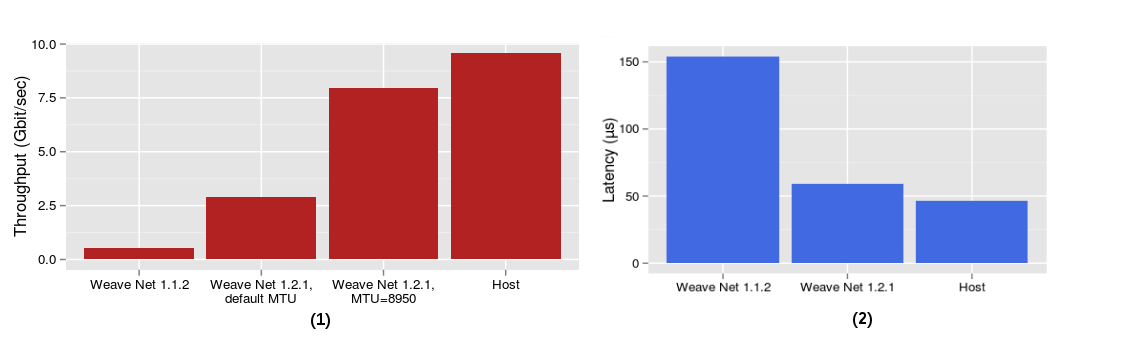
\includegraphics[scale=0.37]{img/weave_perf.png}
	\caption {Performance comparison of Weave versions in terms of throughput (1) and latency (2)}
	\label{fig:weave_perf}
\end{figure}

The developers of Weave and Calico go into more depth and present more detailed results. Wragg \cite{davidwragg2015} evaluated the performance of an older version (1.1) of Weave -which has also been evaluated by Kratzke and Michalek- and the newer version (1.2) which incorporates OVS. Measurements were performed between two Amazon EC2 c3.8xlarge instances \textit{with enhanced networking enabled}. During the experiment, the virtual machines were connected via a 10 Gbps link. Figure \ref{fig:weave_perf} presents the results of the comparison between both Weave versions and native host performance respectively.  Measurements were performed with \texttt{iperf3}. Whilst using the default MTU of 1410 bytes, the performance deterioration of the overall TCP throughput is significant. Wragg attributes these results to a potential bottleneck inside the kernel's network stack. When switching to an MTU size of approximately 9000 bytes (including the VXLAN header) the overall performance is much closer to the performance of the underlying host. He concludes that there is some overhead due to the VXLAN encapsulation which Weave uses, but the results are close to those of host networking. Newer versions of Weave only see a slight decrease in performance and heavily outperform previous versions. Although this performance analysis is executed in a cloud environment, only a single Amazon EC2 availability zone is used. As such, the experiments do not take geographical dispersion into consideration.

White \cite{1_white_2015} presents a performance evaluation of Calico in which he deliberately eliminates the influence of an external network by performing the measurements on two directly connected machines, connected via 10 Gbps interfaces. In this instance the performance is measured with \texttt{qperf}. Figure \ref{fig:calico_perf} presents the results of the throughput and latency measurements. With regards to this research, the bare metal and the container measurements are the main points of interest. Additionally a comparison is made with a standard OpenStack deployment with OVS and VXLAN. The difference in latency between bare metal machines and containers connected with Calico is not significant. However the OVS deployment shows nearly thrice the latency. A similar pattern is seen in the throughput evaluation.   

\begin{figure}[!ht]	
	\centering
	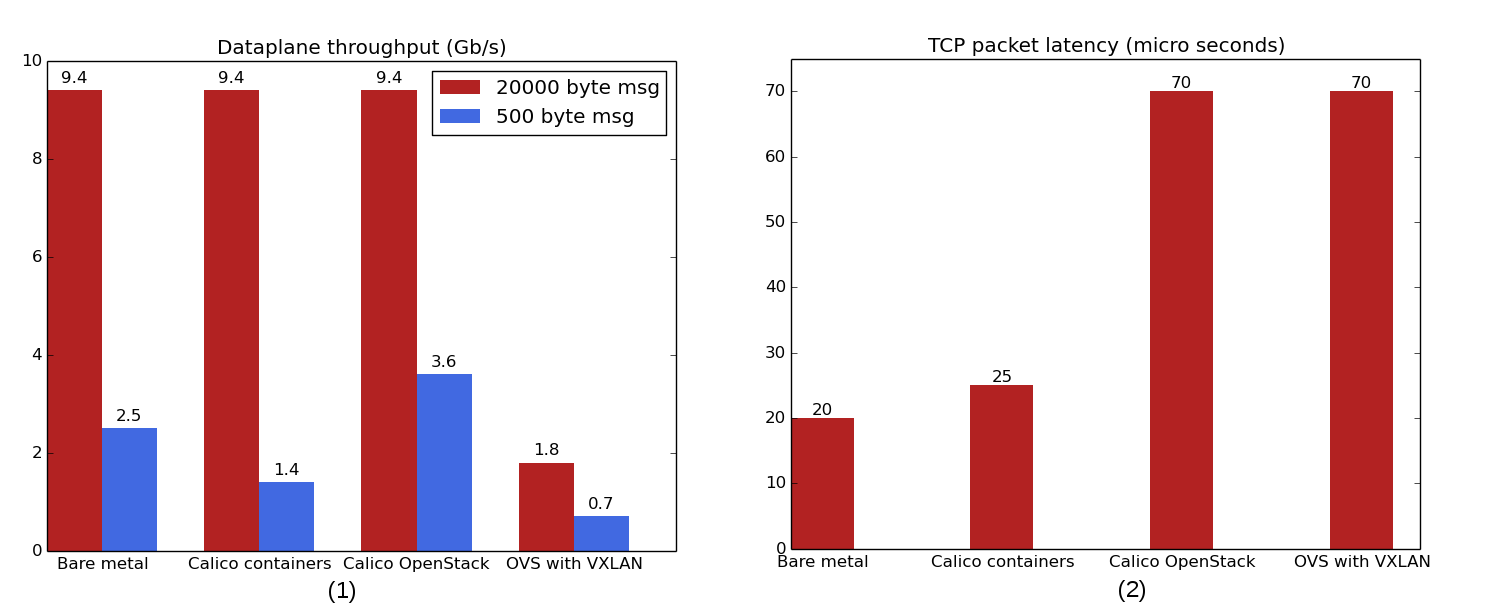
\includegraphics[scale=0.28]{img/calico_perf.png}
	\caption {Performance evaluation of Calico in terms of throughput (1) and latency (2)}
	\label{fig:calico_perf}
\end{figure}

Unrelated to overlay networks, Barker and Shenoy \cite{barker2010empirical} present a series of case studies with which the performance of latency-sensitive applications in a cloud environment can be evaluated. More specifically they present a media streaming setup which resembles a real world scenario. During the course of this project a similar setup will be pursued.

At this point in time, no official research has been performed on the performance of the native overlay driver in \texttt{libnetwork}. Due to the fact that most overlay solutions have restructured their product to work with the modular model of \texttt{libnetwork} nearly all current performance evaluations have become outdated. Moreover, most evaluations exclusively focus on the network performance in a local environment. This paper is a continuation of the work of Claassen and aims to contribute to science by performing a performance analysis of various overlay solutions while factoring in the effects of geographical dispersion. 

